\chapter{Incorporación de una segunda Autoridad de Certificación (FNMT)}
\section{Enunciado}
Carga del segundo certificado de cliente en Firefox. Preferentemente, un certificado FNMT real. Alternativamente, crear una autoridad de certificación nueva, crear un segundo certificado de cliente para el usuario con dicha autoridad e instalarlo en el Firefox. Si se utiliza certificado FNMT, los certificados de autoridad ya se encuentran en el directorio de la máquina Linux (o no) y se deben incorporar a la configuración del Apache.

\section{Resolución}
Para que el servidor Apache acepte certificados de cliente firmados por una segunda autoridad, se ha optado por incorporar la \textbf{AC Raíz FNMT-RCM} como Autoridad de Certificación adicional, junto con la autoridad de la asignatura.

\subsection{Descarga del certificado AC Raíz FNMT-RCM}
Se accede a la sede electrónica de la FNMT (\url{https://www.sede.fnmt.gob.es}) y se descarga el certificado de la \textbf{AC Raíz FNMT-RCM} en formato DER (\texttt{AC\_Raiz\_FNMT-RCM\_SHA256.cer}).

\begin{figure}[H]
    \centering
    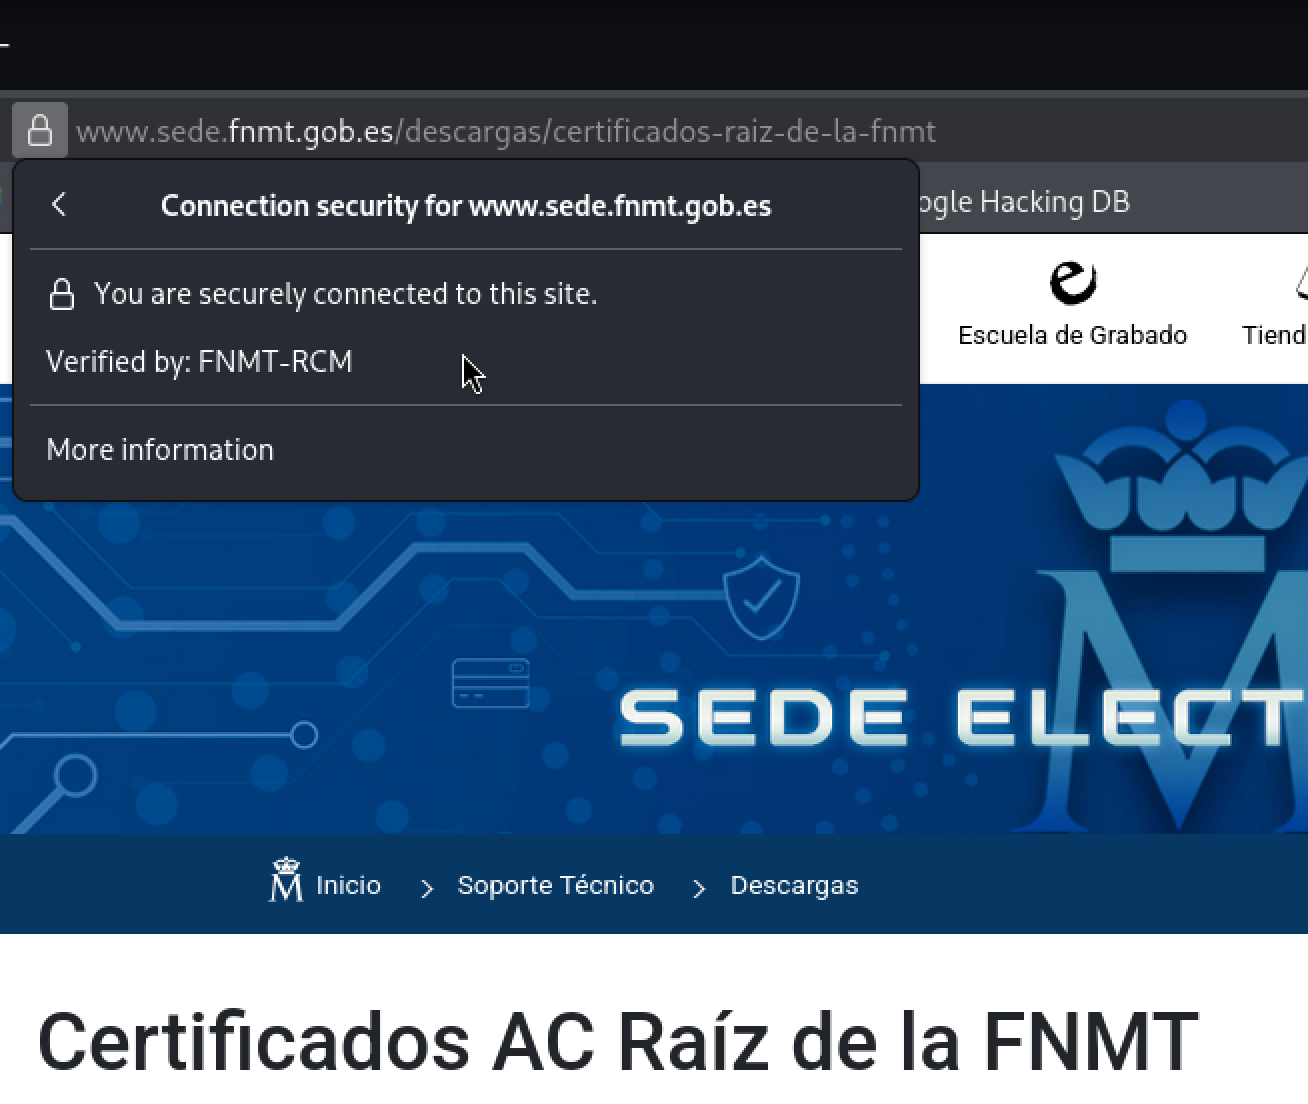
\includegraphics[width=0.7\textwidth]{Imagenes/01-DescargarCAFNMT.png}
    \caption{Página oficial de descarga de la AC Raíz FNMT-RCM.}
    \label{fig:fnmt-descarga}
\end{figure}

\subsection{Verificación de la huella digital (SHA-1)}
Antes de incorporar el certificado al sistema, se comprueba la autenticidad del fichero descargado contrastando su huella SHA-1 contra la publicada por la FNMT en su web oficial.

\begin{lstlisting}[language=bash]
openssl dgst -sha1 AC_Raiz_FNMT-RCM_SHA256.cer
diff <(echo ec503507b215c4956219e2a89a5b42992c4c2c20) \
     <(echo ec503507b215c4956219e2a89a5b42992c4c2c20)
\end{lstlisting}

Al no devolver el comando \texttt{diff} ninguna diferencia, queda verificado que el certificado descargado es íntegro y se corresponde con el publicado por la FNMT.

\begin{figure}[H]
    \centering
    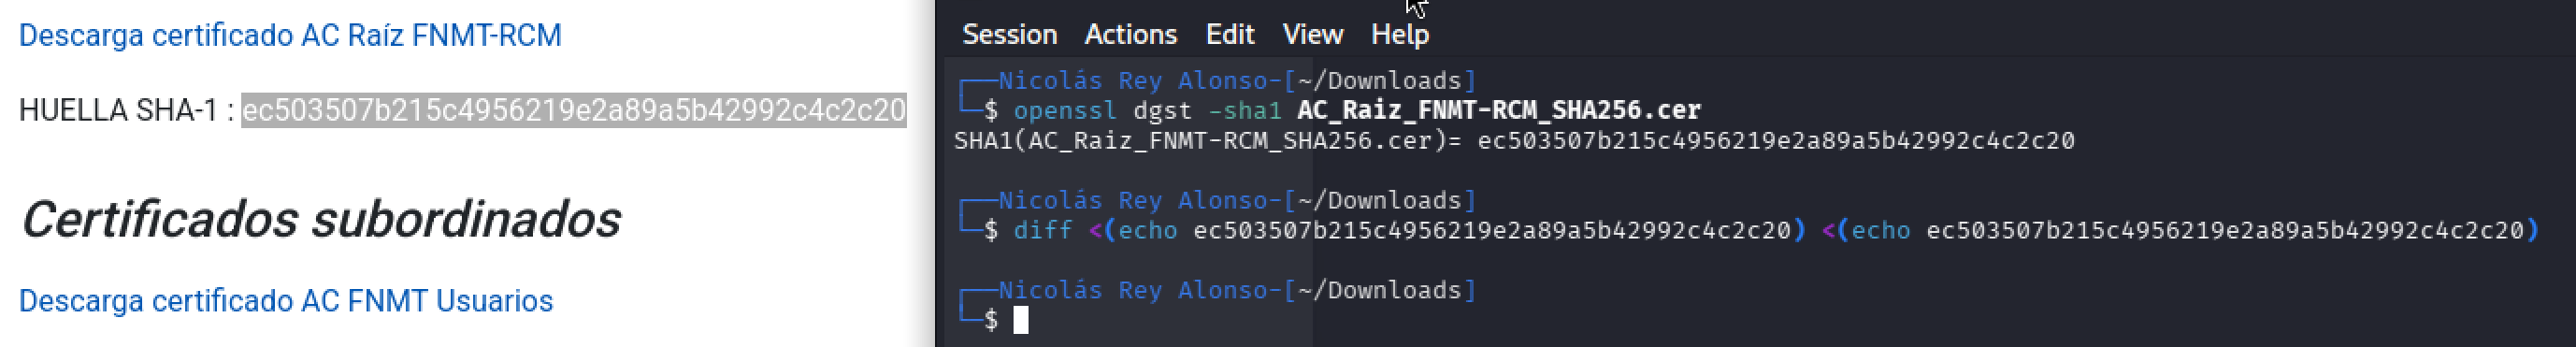
\includegraphics[width=0.95\textwidth]{Imagenes/02-TestVeracityFNMTCA.png}
    \caption{Comparación de la huella SHA-1 publicada con la calculada localmente.}
    \label{fig:fnmt-sha1}
\end{figure}

\subsection{Conversión de DER a PEM}
El certificado se descarga en formato binario DER. Apache requiere los certificados en formato PEM (Base64), por lo que se realiza la conversión con OpenSSL:

\begin{lstlisting}[language=bash]
openssl x509 -inform DER -in AC_Raiz_FNMT-RCM_SHA256.cer \
             -out certificado_fnmt.pem
\end{lstlisting}

\begin{figure}[H]
    \centering
    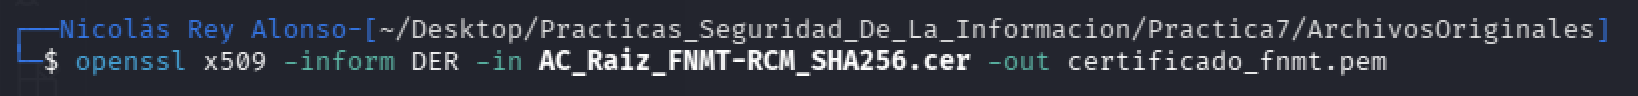
\includegraphics[width=0.95\textwidth]{Imagenes/03-TransformadnCatFNMTandCAULPGC.png}
    \caption{Conversión del certificado raíz FNMT de DER a PEM.}
    \label{fig:fnmt-conversion}
\end{figure}

\subsection{Generación del fichero de CAs confiables}
A continuación, se concatena el certificado de la FNMT con el certificado de la autoridad de la asignatura (\texttt{certificadoRaiz.crt}) en un único fichero PEM que Apache utilizará como almacén de CAs confiables:

\begin{lstlisting}[language=bash]
cat certificado_fnmt.pem certificadoRaiz.crt \
    > ../Salidas/certificados_confiables.pem
\end{lstlisting}

\begin{figure}[H]
    \centering
    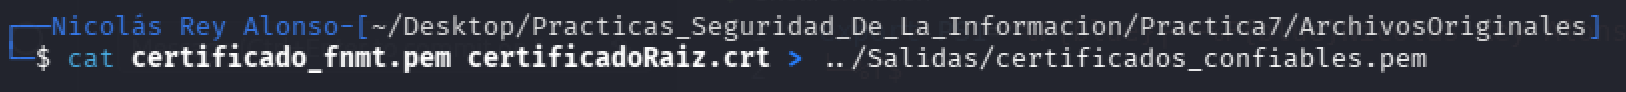
\includegraphics[width=0.95\textwidth]{Imagenes/04-TransformadnCatFNMTandCAULPGC.png}
    \caption{Concatenación del certificado FNMT y de la CA de la asignatura.}
    \label{fig:cat-cas}
\end{figure}

El fichero resultante contiene los dos bloques \texttt{BEGIN CERTIFICATE} / \texttt{END CERTIFICATE}, uno por cada CA reconocida.

\begin{figure}[H]
    \centering
    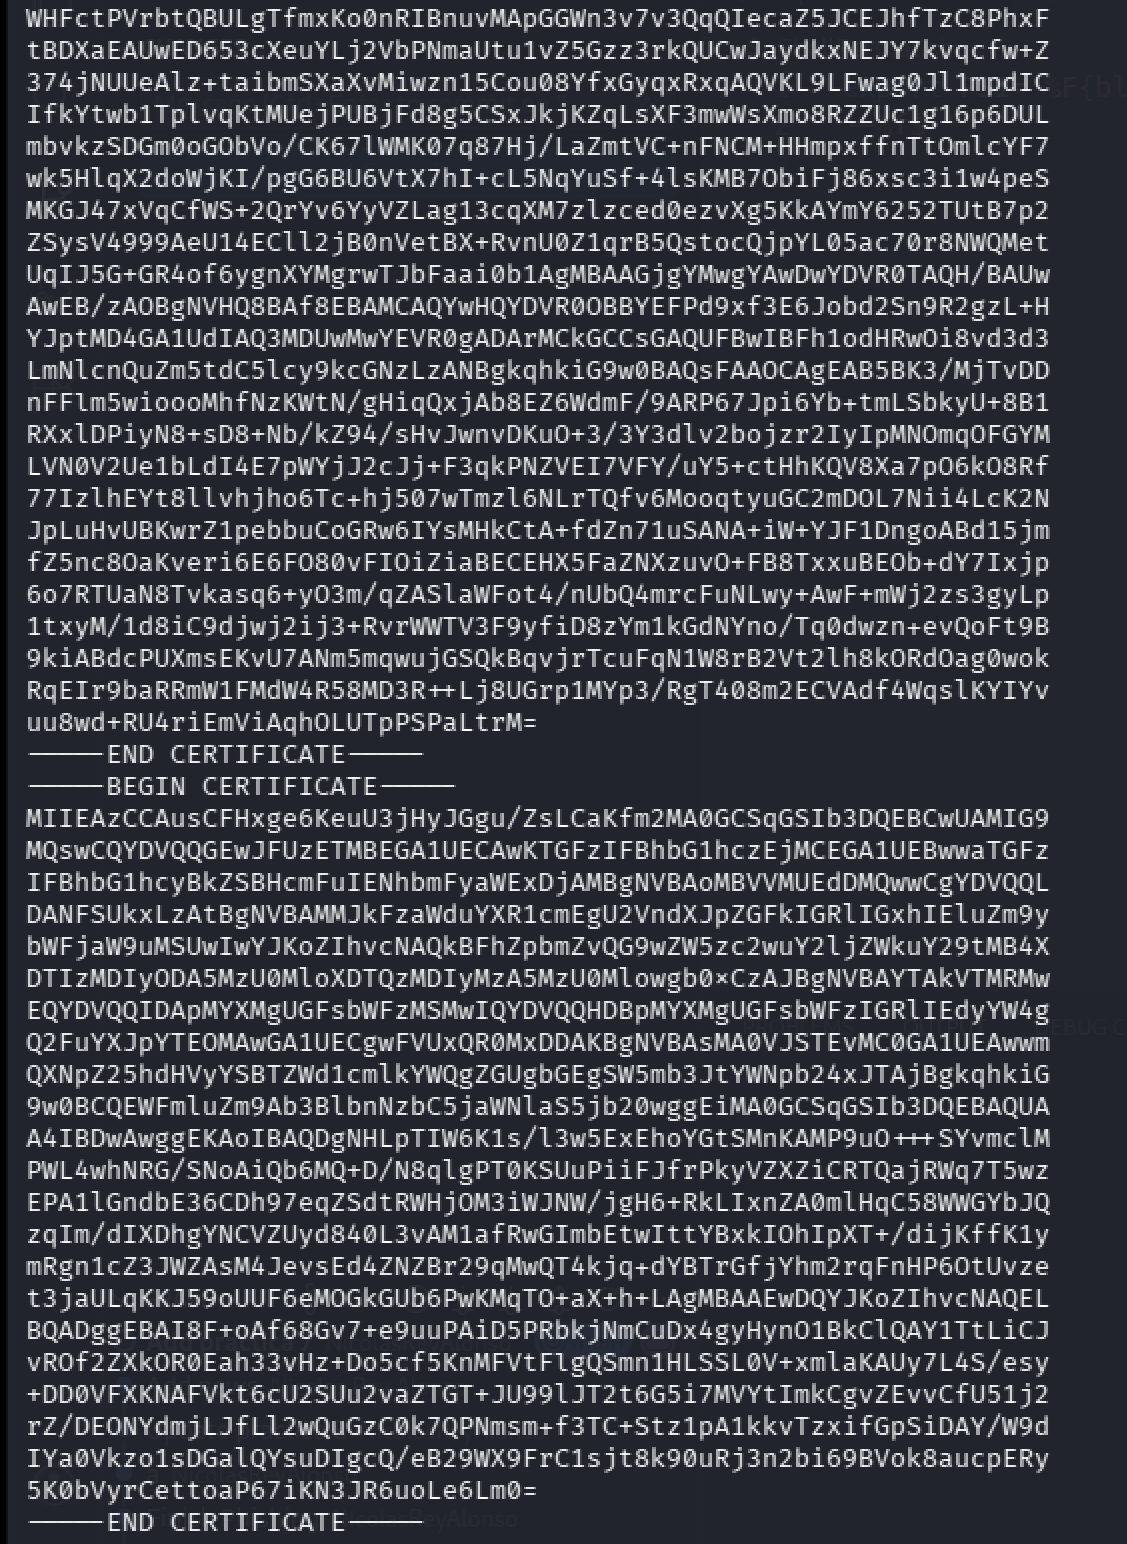
\includegraphics[width=0.7\textwidth]{Imagenes/05-CatFNMT.png}
    \caption{Vista parcial del fichero \texttt{certificados\_confiables.pem}.}
    \label{fig:pem-confiables}
\end{figure}
